\chapter{Updatable Vector Tiles}

\osm{} contributors add more than $3\,000\,000$ nodes and $3\,000\,000$ ways every day.
In order to keep the prerendered tiles up to date this poses a challenge of looking at the changes
and figuring out which tiles are affected by those changes and schedule them for rerendering.

\begin{figure}[H]
  \centering
  \includegraphics[width=0.9\textwidth]{images/updatable_vectortiles_flow.png}
  \caption{Simplified diagram of changed tiles detection process}
\end{figure}

The diagram above shows the simplified process of detecting changed tiles. This chapter will describe how each step is implemented and what problems needed to be solved.

\section{OSM Diff File}

OpenStreetMap provides one huge planet file, which contains every object ever mapped. Since the process of importing is very time and resource consuming it is not feasible to redo this process to keep up with all the changes. Therefore OSM additionally provides Diff files which contain only the created, modified and deleted objects over a period of time. This allows to keep a database in sync with the latest changes. 

\paragraph{Fileformat} The diff file is a compressed XML which contains entries of type create, modify and delete. 

\subsection{Examples}
The example below shows a diff file which contains a create, modify and delete of an OSM object.
\begin{listing}[H]
  \centering
  \begin{xmlcode}
<?xml version='1.0' encoding='UTF-8'?>
<osmChange version="0.6" generator="Osmosis 0.43.1" timestamp="2016-05-20T11:32:32Z">
  <create>
    <node id="4196907493" version="1" uid="1" lat="46.9280366" lon="7.1163806">
      <tag k="amenity" v="pharmacy"/>
      <tag k="name" v="Amavita"/>
    </node>
  </create>
  <modify>
    <node id="4051684660" version="2" uid="1" changeset="..." lat="53.5705074" lon="9.9950888">
      <tag k="emergency" v="fire_hydrant"/>
      <tag k="ref" v="13874"/>
    </node>
    </modify>
  <delete>
    <node id="1044604768" version="2" uid="1" changeset="..." lat="52.6429848" lon="5.082264"/>
  </delete>
</osmChange>
  \end{xmlcode}
  \caption{Create, modify and delete}
\end{listing}

\subsection{Different change scenarios}

\paragraph{Adding an object} This is the default scenario an object gets added.

\paragraph{Deleting an object} An object gets deleted for example an old house which does not exist anymore.

\paragraph{Modifying an object} An object gets modified for example additional translations get added to a place.

\paragraph{Moving an object} An objects is moved for example a bus stop was not correctly mapped or was moved in the real world. This is a modify where all tags stay the same but the longitude and latitude value of the node change.

\section{Diff Import and Tracking of Changed Rows}

Imposm3 is used for the regular import of the OSM Planet file. Additionally it supports importing OSM Diff files. Imposm3 will read the XML File and creates the geometries out of the node, way and relation objects. A create entry will result in an sql insert, a delete entry results in an sql delete however a modify entry results an sql delete and sql insert statement.\\\\
The diff import functionality of imposm3 is only meant to keep the database in sync with the osm changes. It is not possible to track which rows in the table has been inserted, updated or deleted. This extra functionality which is later needed to calculate the affected tiles had to be implemented.\\\\
The first implementation used insert and delete triggers to track which columns where inserted and deleted. After testing this solution on a planet scale it turned out that with multiple millions creates, modifies and deletes the trigger solution was just too slow.\\
So a different solution was developed which modified the imposm3 implementation to additionaly set a timestamp column in the insert statatement. This solution was performing very well but did not cover the case of deleting objects. As this would just be deleted and could not be tracked later on. Specially for the deleted objects the triggers were used. This resulted in a satisfying  performance. 

\paragraph{Meaning of satisfying performance} In order to be able to keep up with rendering changes the update process can not take longer than the number of days the database is behind.

\subsection{Track changes}

\subsubsection{Track inserted and updated rows}


\subsubsection{Track deleted rows}

For each table the \texttt{track\_osm\_delete} trigger is enabled to keep track of deleted rows.

\begin{listing}[H]
  \centering
  \begin{sqlcode}
    DROP TRIGGER IF EXISTS osm_building_polygon_track_delete ON osm_building_polygon;
    CREATE TRIGGER osm_building_polygon_track_delete
    BEFORE DELETE ON osm_building_polygon
    FOR EACH ROW EXECUTE PROCEDURE track_osm_building_polygon_delete()
  \end{sqlcode}
  \caption{Delete trigger on a table}
\end{listing}

The trigger will track the delete in a separate table before discarding it.

\begin{listing}[H]
  \centering
  \begin{sqlcode}
CREATE OR REPLACE FUNCTION track_osm_building_polygon_delete() returns TRIGGER
AS $$
BEGIN
     IF (TG_OP = 'DELETE') THEN
        INSERT INTO osm_building_polygon_delete(id, geometry)
        VALUES($1, $2) USING OLD.id, OLD.geometry;
        RETURN OLD;
     END IF;

     RETURN NULL;
END;
$$ language plpgsql;

  \end{sqlcode}
  \caption{Logic of delete trigger}
\end{listing}


%----------------------------
\newpage{}
\section{Calculate changed tiles}

One way to determine which tiles are affected by changes in the database is to calculate the covered tiles by all changed geometries by recursively descending the XYZ Quadtree and checking for intersections of the tiles and geometries.

\subsubsection*{Algorithm}

\begin{enumerate}  
    \item \label{itm:calc-extent}Calculate the extent $e$ for a given XYZ tile index $i$
    \item \label{itm:bbox} Check if geometry $g$ intersects with the tile extent $e$
    \item Select tile index $i$ if \ref{itm:bbox} is successful
    \item Stop if max zoom level $Z$ has been reached
    \item Call \ref{itm:calc-extent} for all four children of $i$ if \ref{itm:bbox} is successful
\end{enumerate}

\begin{figure}[H]
  \centering
  \includegraphics[width=0.9\textwidth]{images/polygon_xyz_matching.png}
  \caption{Recursive tile matching on polygon}
\end{figure}

\subsubsection*{Tile Buffers}

Vector tiles are utilizing buffers to ensure nice geometry joining. To support this feature the algorithm has been adapted to add a buffer to the bounding box of the tile.

\begin{figure}[H]
  \centering
  \includegraphics[width=0.7\textwidth]{images/polygon_buffer_xyz_matching.png}
  \caption{Recursive buffered tile matching on polygon}
\end{figure}


\subsubsection*{PostgreSQL Implementation}

The PostGIS implementation makes heavy use of the \texttt{&&} operator and GiST indizes on the geometry columns to check whether the tile extent and geometry intersect with each other. Although using the bounding box of the geometry is not accurate and can yield false positive changed tiles it is much faster than using the correct \texttt{ST\_Intersects}.

\begin{listing}[H]
  \centering
  \begin{sqlcode}
CREATE OR REPLACE FUNCTION overlapping_tiles(geom geometry, max_zoom_level INT, buffer_size INT)
RETURNS TABLE (tile_z INT, tile_x INT, tile_y INT) AS $$
BEGIN
    RETURN QUERY
        WITH RECURSIVE tiles(x, y, z, e) AS (
            SELECT 0, 0, 0, geom && XYZ_Extent(0, 0, 0, buffer_size)
            UNION ALL
            SELECT x*2 + xx, y*2 + yy, z+1,
                   geom && XYZ_Extent(x*2 + xx, y*2 + yy, z+1, buffer_size)
            FROM tiles, (VALUES (0, 0), (0, 1), (1, 1), (1, 0)) as c(xx, yy)
            WHERE e AND z < max_zoom_level
        )
        SELECT z, x, y FROM tiles WHERE e;
END;
$$ LANGUAGE plpgsql IMMUTABLE;
  \end{sqlcode}
  \caption{Recursive tile matching of geometry}
\end{listing}


\section{Point Optimization}

Points only occur in one tile at each zoom level (neglecting tile buffers). 

\begin{figure}[H]
  \centering
  \includegraphics[width=0.9\textwidth]{images/point_xyz_matching.png}
  \caption{Tiles covering a point geometry}
\end{figure}

Therefore given a point we can immediately calculate the tile it is covering saving the recursive descend.
To neglect overhead of PostgreSQL dynamic language a PostgreSQL C extension has been written which improves tile calculation for points a hundred fold.

\begin{listing}[H]
  \centering
  \begin{ccode}
#include "math.h"
float8 D2R = M_PI / 180.0;

// Latitude and longitude of Zurich
int32 zoom_level = 14;
float8 lat = 47.376887;
float8 lon = 8.541694;

float8 _sin = sin(lat * D2R);
float8 z2 = pow(2, zoom_level);

// XYZ Tile index calculated from latitude and longitude
int32 x = floor(z2 * (lon / 360 + 0.5));
int32 y = floor(z2 * (0.5 - 0.25 * log((1 + _sin) / (1 - _sin)) / M_PI));

  \end{ccode}
  \caption{Calculate tile at given zoom level for a point}
\end{listing}

Applying the \texttt{overlapping\_tiles} function over millions of polygons is very efficient thanks to the new \texttt{LATERAL} join type.

\begin{listing}[H]
  \centering
  \begin{sqlcode}
    SELECT DISTINCT t.tile_x AS x, t.tile_y AS y, t.tile_z AS z
    FROM osm_building_polygon AS g
    INNER JOIN LATERAL overlapping_tiles(g.geometry, 14, 4) AS t ON true
  \end{sqlcode}
  \caption{Calculate all tiles covered by building polygons}
\end{listing}

\begin{figure}[H]
  \centering
  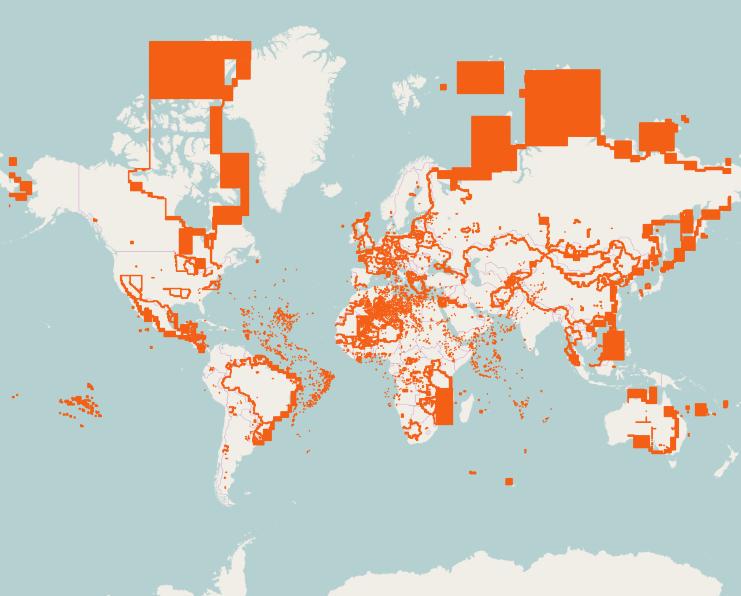
\includegraphics[width=1\textwidth]{images/changed_tiles_z10.png}
  \caption{Changed tiles on z10 over course of 10 days}
\end{figure}
